\newpage
\chapter{Implementatie}

\par In de volgende hoofdstukken wordt besproken hoe het eindresultaat bereikt werd. De werkwijze is stapsgewijs en in elke stap wordt er verder geoptimaliseerd. In de eerste stappen was er nog sprake van een kleurenconversie van YCbCr naar RGB, maar deze werd later weggelaten om aan snelheid te winnen. In het definitieve ontwerp wordt dus volledig gewerkt in de YCbCr kleurenruimte met het oog op de snelheid van de frameprocessing.

\section{Algemeen overzicht}

	\begin{figure}[H]
			\centering
			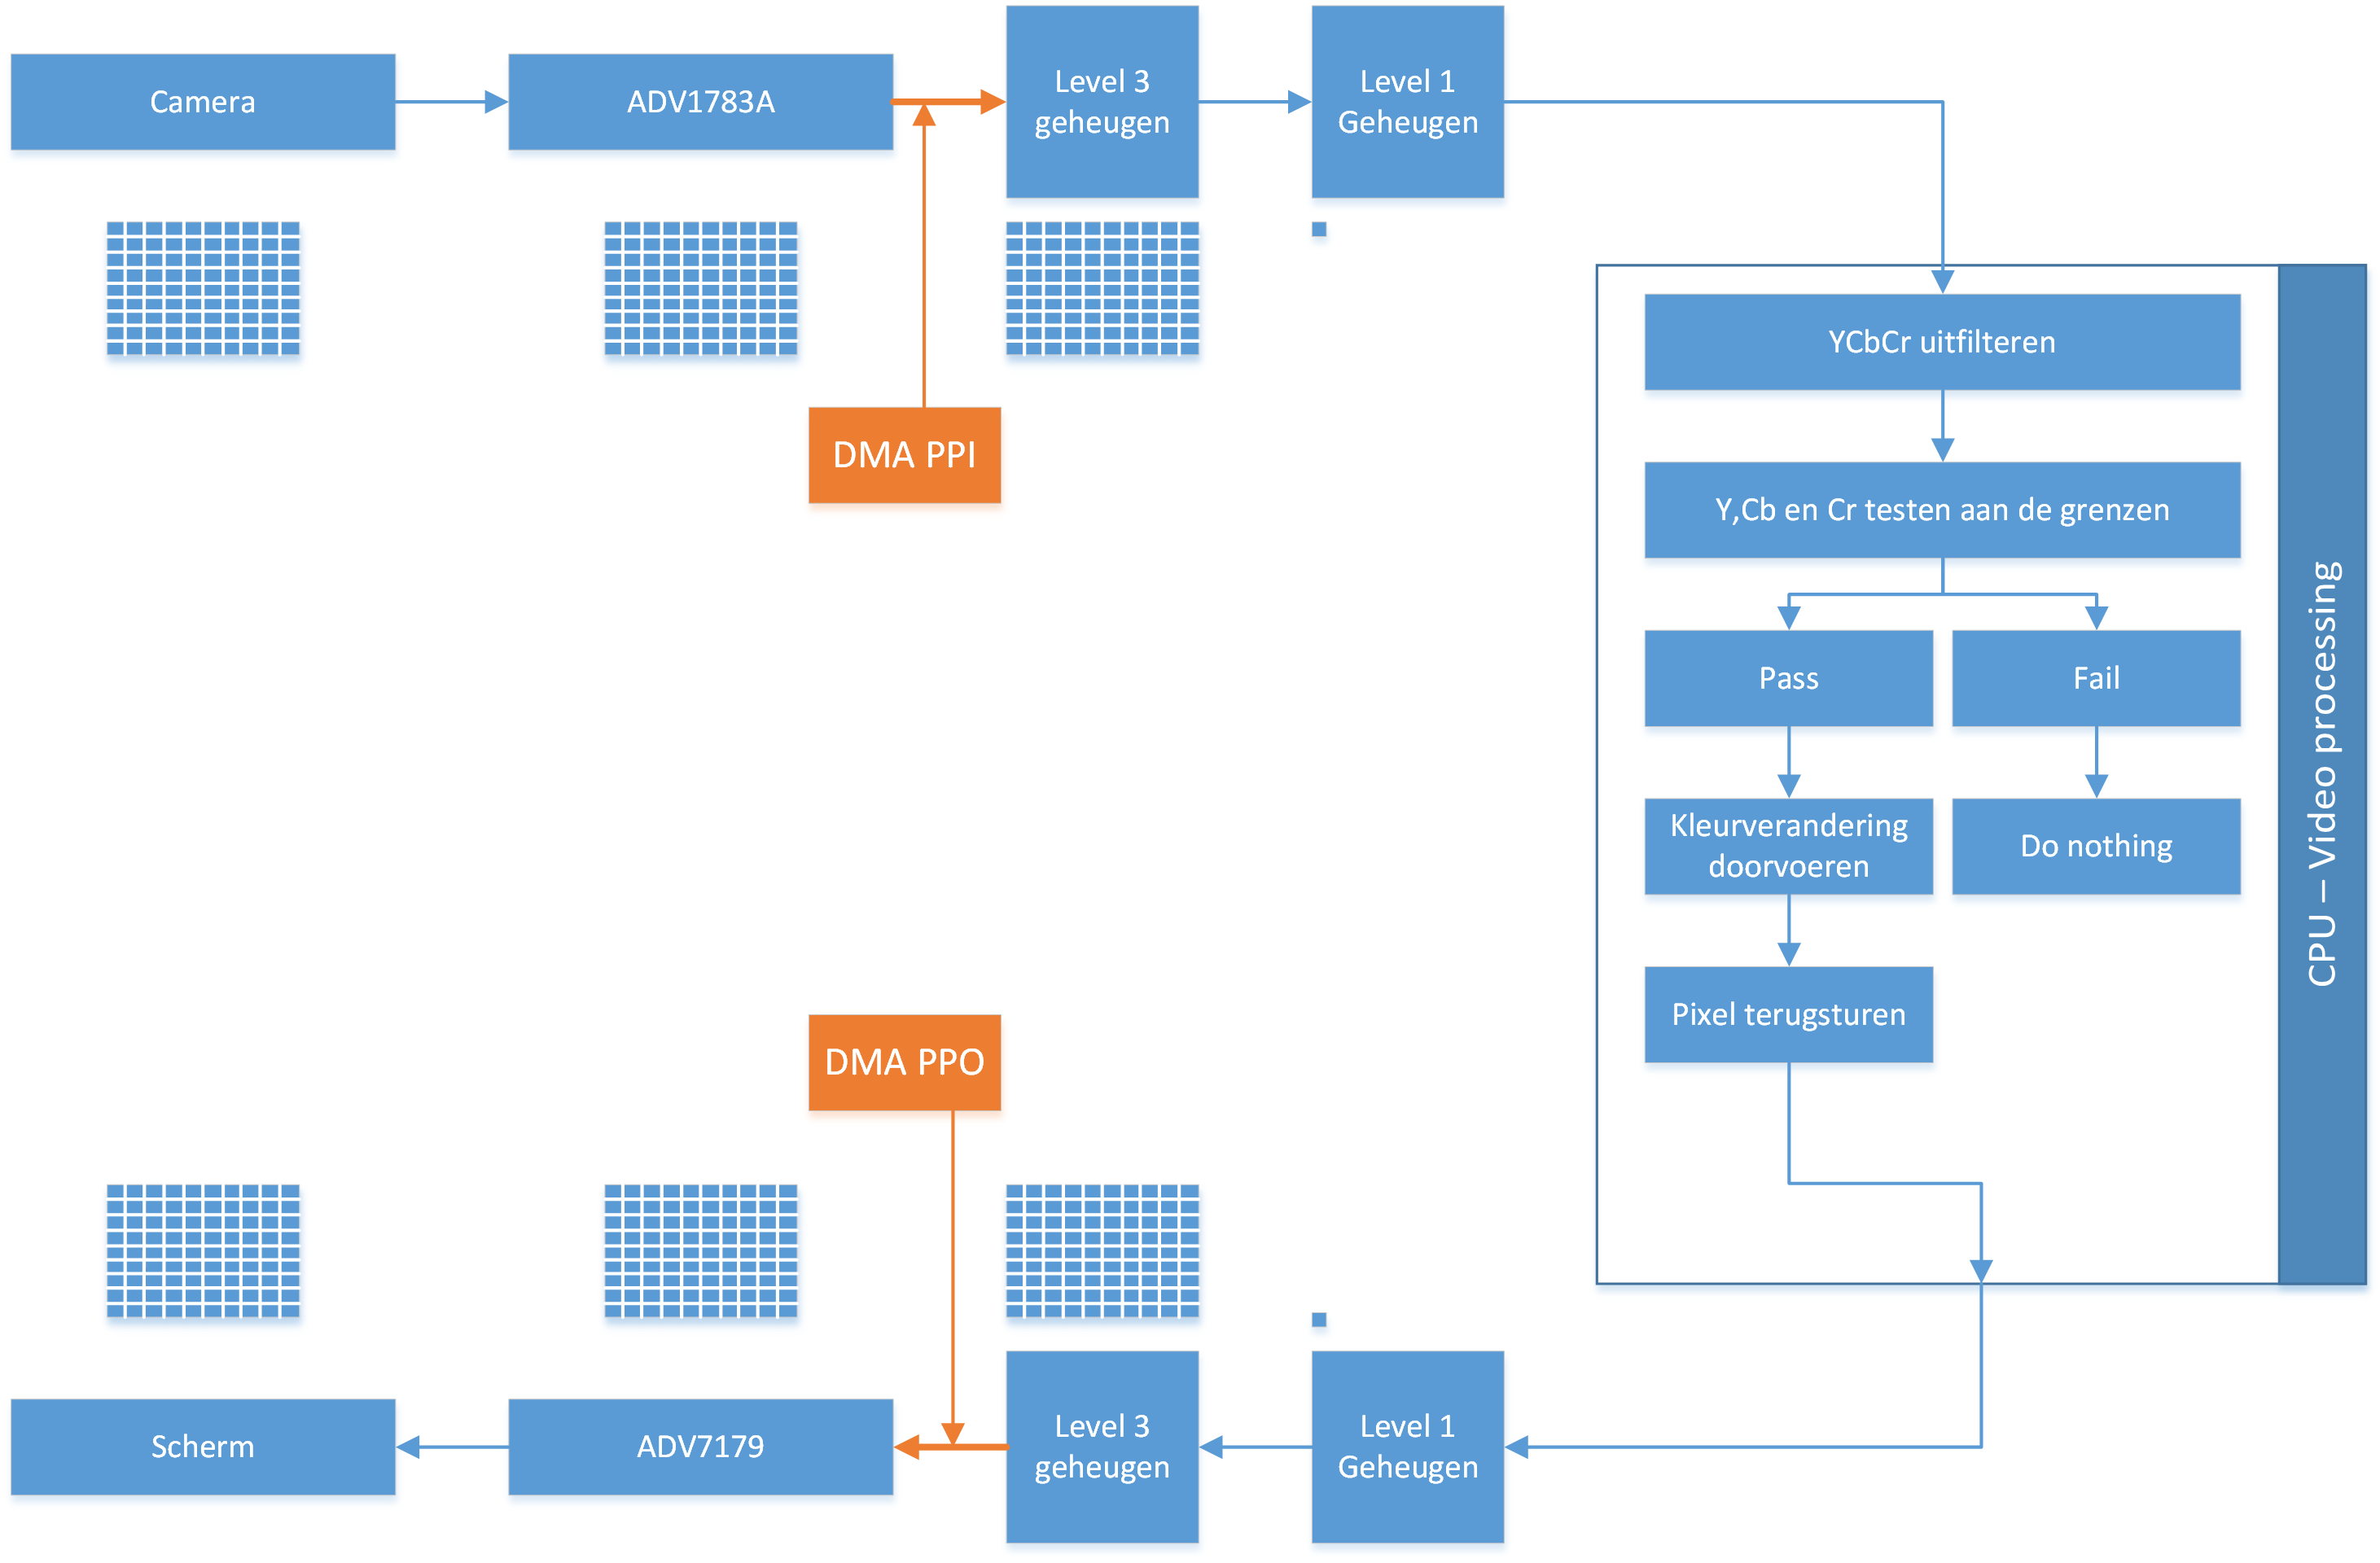
\includegraphics[width=1.0\textwidth]{Chapters/Chapter2/Images/implementationOverview.png}
			\caption{Algemeen overzicht van de implementatie op de BlackFin BF-561}
			\label{fig:algemeenoverzicht}
	\end{figure}
	\newpage
	\par Het algemeen opzet van de implementatie van het algoritme wordt weergegeven in figuur~\ref{fig:algemeenoverzicht}. Deze figuur is eveneens terug te vinden in appendix~\ref{app:algemeenoverzicht}. De videodata wordt binnengelezen van een digitaal fototoestel en via de video decoder die op het EZ-kit aanwezig is wordt deze videodata door middel van PPI opgeslagen in het level 3 SDRAM geheugen. Vervolgens zal door de processor telekens 1 pixel opgevraagd worden om verwerkt te worden. Deze pixel wordt dan gekopieerd naar het level 1 geheugen. Hierna wordt het verwerkingsalgoritme toegepast op de pixel. Dit algoritme zal in de hoofdstukken hieronder verder worden besproken. Indien de pixel van waarde veranderd is na toepassing van het algoritme, dan zal deze terug van het level 1 geheugen naar het level 3 geheugen gestuurd worden. Via de PPO wordt het beeld vervolgens van het level 3 geheugen naar de video encoder gezonden die op zijn beurt het videosignaal doorgeeft aan een scherm.

\section{Frame iteratie}
	\subsection{Active Video Frame}
		\par Om de AVFs te kunnen vinden, moeten we tweemaal met een verschillende offset door de array itereren. Aangezien een lijn ook nog bytes bevat waar men beter niets aan veranderd, is de eenvoudigste oplossing te itereren over de lijnen binnen een frame, en dus telkens de lijnindex te vermenigvuldigen met de lijnlengte (dit is hier 1716 bytes). In elke iteratie van deze loop verkrijgen we een nieuwe lijn. Het eerste AVF bevat de oneven lijnen, en dus zijn dit ook de eerste die we zullen bewerken.
		\smallskip
		\begin{lstlisting}[language=C,caption=Code voor het itereren over een frame]
#define AVSTART1 20
#define AVSTART2 281

for(int avField = 0; avField<2; avField++)
{
	int startFor = (avField==0)?AVSTART1:AVSTART2;
	int endFor = startFor+((avField==0)?AVLENGTH1:AVLENGTH2);
	for(int i=startFor; i<endFor; i++)
	{
		//...
	}
}		\end{lstlisting}

	\subsection{Processing van een beeldlijn}
		\par Een lijn bevat eerst 276 bytes data die we niet mogen overschrijven (Cfr.~\ref{subsec:LijnSubSec}). Pas daarna volgen de 1440 bytes data die wij moeten uitlezen en bewerken. We lezen per iteratie 4 bytes uit omdat deze alle 4 nodig zijn om twee volledige pixels te kunnen bepalen en te converteren naar RGB. Dit zorgt er voor dat we per twee over de array lopen:
		\smallskip
		\begin{lstlisting}[language=C,caption=Code voor her itereren over een lijn]
#define LINEOFFSET 276/2		// 4 EAV + 268 HB + 4 SAV
#define LINELENGTH 1716/2		// ITU-R BT656 line is 1716 bytes

for(j=LINEOFFSET; j<LINELENGTH; j+=2)
{
	//...
}		\end{lstlisting}

\section{Kleurenconversie}
	\subsection{YCbCr naar RGB}
		\par Zoals reeds aangegeven in~\ref{subsec:KleurConversieSubSec}, kunnen we YCbCr perfect converteren naar RGB als we beschikken over vier bytes data die respectievelijk Cb, Y1, Cr en Y2 voorstellen. De input komt binnen onder de vorm van twee shorts, waaruit CbY en CrY gehaald moeten worden. Om dit te bereiken zijn er twee operaties vereist, namelijk shiften en masken, en dit voor beide shorts. Aan de hand van de formules op pagina~\pageref{tab:RGBYCbCrFormulesTable} kunnen we de 4 verkregen bytes omrekenen tot RGB waarden, of in C code:
		\smallskip
		\lstinputlisting[language=C++,caption=YUV naar RGB conversie ge\"implementeert op de BF-561]{Chapters/Chapter2/SourceCode/YUVtoRGB.c}

		\par We cre\"eren een functie die de twee short als argumenten verkrijgt, en na een aantal operaties een jagged array teruggeeft met daarin twee RGB pixelwaarden. Zoals zichtbaar is moet er, om de Cb en Cr te bepalen eerst 8 bit geshift worden naar links. Dit is vereist aangezien ze werwerkt zit in de eerste 8 bits van de short. Om geen onverwachte resultaten te bekomen masken we nog eens met 0xFF zodat we zeker zijn dat de eerste bits allemaal op 0 staan en dus het resultaat niet kunnen be\"invloeden. Om Y1 en Y2 te bepalen is enkel de mask nodig die we als de laatste stap op Cb en Cr ook toegepast hebben. Als laatste combineren we de verkregen waarden in een array en geven deze terug naar waar de aanroep plaatsvond.

	\subsection{RGB naar YCbCr}
		\par RGB naar YCbCr is een heel wat complexere operatie dan de omgekeerde. Dit omdat het berekenen van Y, Cb en Cr een groter aantal operaties vergt. We maken opnieuw een functie, maar ditmaal ontvangt ze de jagged array die gegenereerd wordt in de YCbCr naar RGB conversie als argument, en geeft ze een array van 2 shorts terug, die dan de 2 pixels voorstellen in de YCbCr kleurenruimte.
		\smallskip
		\lstinputlisting[language=C++,caption=todo]{Chapters/Chapter2/SourceCode/RGBtoYUV.c}

		De berekening om de RGB waarden om te zetten naar YCbCr is te vinden in de tabel~\ref{tab:RGBYCbCrFormulesTable} op pagina~\pageref{tab:RGBYCbCrFormulesTable}. Deze passen we toe op de RGB waarden in de binnenkomende array. Deze array is van het formaat {{R,G,B},{R,G,B}} en bevat dus telkens twee pixels. Als laatste stap moeten we de Y, Cb en Cr waarden samenvoegen tot twee shorts die respectievelijk CbY en CrY voorstellen. Om Cb toe te kennen aan de hoogste 8 bit van de short, stellen we CbY eraan gelijk en shiften we ditmaal 8 bits naar links, dus te tegenovergestelde operatie als in de YCbCr naar RGB conversie. Daarna tellen we Y erbij op om deze in de laagste 8 bits te plaatsen. Deze handeling doen we tweemaal, om beide pixels geconverteerd te hebben.

\section{Eerste iteratie}
	\par Nu we de conversies apart bekeken hebben, en ook de iteratie over het frame volledig beschreven hebben, zijn we in staat om dit samen te voegen tot \'e\'en werkend geheeld. Deze code is toegevoegd in bijlage~\ref{app:codesnippet1} op pagina~\pageref{app:codesnippet1}. Het probleem dat zich manifesteerde bij het analyseren van deze code was dat de processing tijd per frame te lang was. Hierdoor verkregen we als uitvoer een flikkerend onstabiel beeld. Er werd gezocht naar een oplossing.

\section{Tweede iteratie}
	\par In een tweede iteratie werd als eerste de conversie van RGB naar YCbCr en omgekeerd verwijderd uit het proces. Dit leverde al een aanzienlijke snelheidswinst op, maar in het worst case scenario waarbij getest werd met een volledig blauw beeld werd slechts 1/4 van het scherm van kleur veranderd. Er is dus meer tijd nodig om een frame volledig te verwerken. Twee mogenlijkheden boden zich aan:

		\begin{enumerate}
			\item Het toepassen van interleaving op de lijnen van het frame. Dit houd in dat in een eerste frame enkel de even lijnen verwerkt worden en in een tweede frame enkel de oneven lijnen.
			\item Het vergroten van de framebuffer geeft de processor meer tijd om een frame te verwerken. Het huidige aantal buffers was 4.
			\item Het samennemen van naast elkaar liggende pixels, om zo het oog te bedriegen.
		\end{enumerate}

	\par Er werd gekozen voor de 2\textsuperscript{e} mogelijkheid. De buffer werd eerst vergroot naar 8 frames, maar dit bleek nog steeds niet voldoende. Wanneer een volledig blauw scherm aanlegden als videosignaal was de verkregen verwerkingstijd nog steeds te kort. Hierna werd overgeschakeld naar een buffering van 32 frames. De verwerkingstijd werd nu aanzienlijk vergroot. Als nadeel daalde de framerate met factor 4. De frame processing code aangepast zoals te zien is in bijlage~\ref{lis:video_A.c}.

	\par De derde mogelijkheid, die ervoor zorgt dat door het checken van een enkele pixel er meerdere pixels tegelijk aangepast worden, was perfect mogelijk en hebben we ook toegepast op deze code. Aan het resultaat was duidelijk te zien dat er een versnelling was in de verwerkingstijd, maar ook dat de resolutie van het schemr als het ware gedeeld werd door 4. Het werkt namelijk zo: er wordt ge\"itereerd over het frame zoals reeds gebeurde, ditmaal echter verspringt de teller steeds per 2 pixels per lijn. Op die manier wordt er dus telkens een pixel overgeslagen. Indien een pixel voldoet aan de eisen om van kleur verandert te worden, worden de naast-, onder- en rechtonderliggende pixels ook meteen vervangen. Dit wil dus ook zeggen dat we enkel de oneven lijnen moeten doen. Zo kan de totale iteratietijd gedeeld worden door 4. De uiteindelijke resolutie is echter zo erbarmelijk dat we besloten dit niet in de uiteindelijke code te behouden.Aangezien we de code geschreven hebben, en ze ook effectief werkt, is ze te zien in bijlage~\ref{lis:video_A_block.c}.

	\par In de code in bijlage~\ref{lis:video_A.c} is niet alleen de kleurenconversie verdwenen, maar is ook een optimalisatie uitgevoerd om het aantal for-iteraties te verminderen. Zo worden AV field 1 en AV field 2 in eenzelfde for-iteratie overlopen. Van de 32 buffers die ter beschikking staan worden er slechts 8 overlopen om de processor meer tijd te geven om deze verwerking te voltooien. Hieraan is ook de framerate verlaging met factor 4 te wijten.

	\par Om deze buffering te vergroten, zijn meer aanpassingen nodig dan enkel in de source files. De buffers worden namelijk op vaste adressen geplaatst om en zo ideaal mogelijk systeem te bekomen. Aangezien het aantal buffers sterk gestegen is, moet deze mapping volledig herzien worden, en dit gebeurt in de linker file. Om het overzicht te bewaren zijn enkel de regels die aangepast zijn weergegeven in bijlage~\ref{lis:video_in_out.ldf}. Daar is te zien hoe er 32 banken voorzien worden van elk 2MB groot. De verklaring voor deze grootte is te lezen in hoofdstuk~\ref{sec:dmacontroller}.
	De frames waarin de data opgeslagen wordt bevinden zich in in het level 3 geheugen, dus ook daar moeten aanpassingen gebeuren. Deze aanpassingen bevinden zich in de files L3\textunderscore SDRAM.h, L3\textunderscore SDRAM.c en uiteindelijk ook system.h. De bekomen code is te zien in respectievelijk bijlagen~\ref{lis:L3_SDRAM.h}, ~\ref{lis:L3_SDRAM.c} en ~\ref{lis:system.h}.

	\par Bronnen:~\cite{bib_12},~\cite{bib_13},~\cite{bib_11}